 %!TEX root = ../dissertation.tex
%\begin{savequote}[75mm]
%This is some random quote to start off the chapter.
%\qauthor{Firstname lastname}
%\end{savequote}

\chapter{Approximating Bayesian inference}
\label{chap:approx}

This chapter provides a brief introduction to the approximate inference methods that will be used throughout this thesis. These form the backbone of most rational process models for human cognition, as well as of algorithms for machine intelligence in a structured probabilistic models framework. First, I introduce the computational problem we hope to approximate and explain why it is challenging. Second, I introduce sampling-based approaches, focusing on methods based on Markov chains. Third, I introduce variational approaches to this problem. Finally, I briefly discuss the trade-offs between these two methods, and how they might be combined.

\section{The challenge of Bayesian inference}
Bayesian inference is a method in statistics where Bayes' theorem is used to update the probabilities of hypotheses $h \in \mathcal{H}$ (where $\mathcal{H}$ specifies the space of possible hypotheses) as more information or data $d \in D$ (where $D$ represents the space of values observed data can take) is made available. We consider a simple coin-flipping example: here we wish to update the probabilities that a coin is biased towards Heads ($h_1$), is biased towards Tails ($h_2$), or unbiased ($h_0$) based on observing the results of coin flips ($d \in \{\text{H}, \text{T}\}$ for heads or tails). Bayesian inference has two key components each together form a statistical model for the observed data. First, a prior distribution $P(h)$ defined over all hypotheses $h \in \mathcal{H}$ that determines the a priori probability of a certain hypothesis. In our coin flipping example, without any data, we are likely to have a fairly high expectation that a coin is generally unbiased. This gives high prior probability to $h_0$, and lower prior probabilities to $h_1$ and $h_2$. Second, a likelihood function $P(d | h)$ that defines the probability of observing different kinds of data given, specific hypotheses. So in our coin-flipping example, the likelihood is a Bernoulli probability distribution given by $P(\text{H} | h) = q = 1 - P(\text{T} | h) = 1- q$ with different parameters $q$ for the hypotheses $h_0, h_1$ and $h_2$. The goal then is to combine these two pieces of information -- a priori knowledge via the prior distribution, as well as information from the data observed via the likelihood function -- to form a \textit{posterior probability distribution} over the hypotheses. This is represented as $P(h | d)$ and computed using Bayes' rule as follows:

\begin{align}
    P(h|d) = \frac{P(d, h)}{\sum_{h'} P(d, h')} = \frac{P(d|h)P(h)}{\sum_{h'} P(d|h') P(h')}
\end{align}

The numerator i.e. the joint distribution over the data and the hypothesis is easy to compute since we already know the two components -- the prior and the likelihood, and these just need to be multiplied. The denominator however requires a summation over all the possible hypotheses. This is tractable in our coin-flipping case since, in the specific and limited way in which we have formalized the problem, the space of hypotheses is very small (3 possibilities). However, for several problems of practical significance -- including many that humans solve everyday -- this summation (or integral) is intractable.\footnote{There exist priors and likelihoods such that this integral remains tractable even for large or continuous hypothesis spaces. These are called conjugate families of prior and likelihood. However, many real world data generating processes cannot be well approximated by distributions from such conjugate families.}  For example, consider a clinician diagnosing a patient. A patient can simultaneously have any of $N$ possible conditions. This means that the hypothesis space contains $2^N$ hypotheses. Or consider the segmentation problem, faced constantly by the visual system, of assigning each retinotopic location to the surface of an object. If there are $K$ objects and $N$ locations, the hypothesis space contains $K^N$ hypotheses. Such vast hypothesis spaces render exact computation of Bayes' rule intractable, because the denominator (the normalizing constant, sometimes called the partition function or marginal likelihood) requires summation over all possible hypotheses. Computing this normalization constant is the key computational challenge in Bayesian inference, and computing exact posterior probabilities of hypotheses. In the following sections, I will introduce the two main approaches to approximating such posteriors.

\section{Monte Carlo methods}
\label{sec:approx_MC}

\begin{figure}
\centering
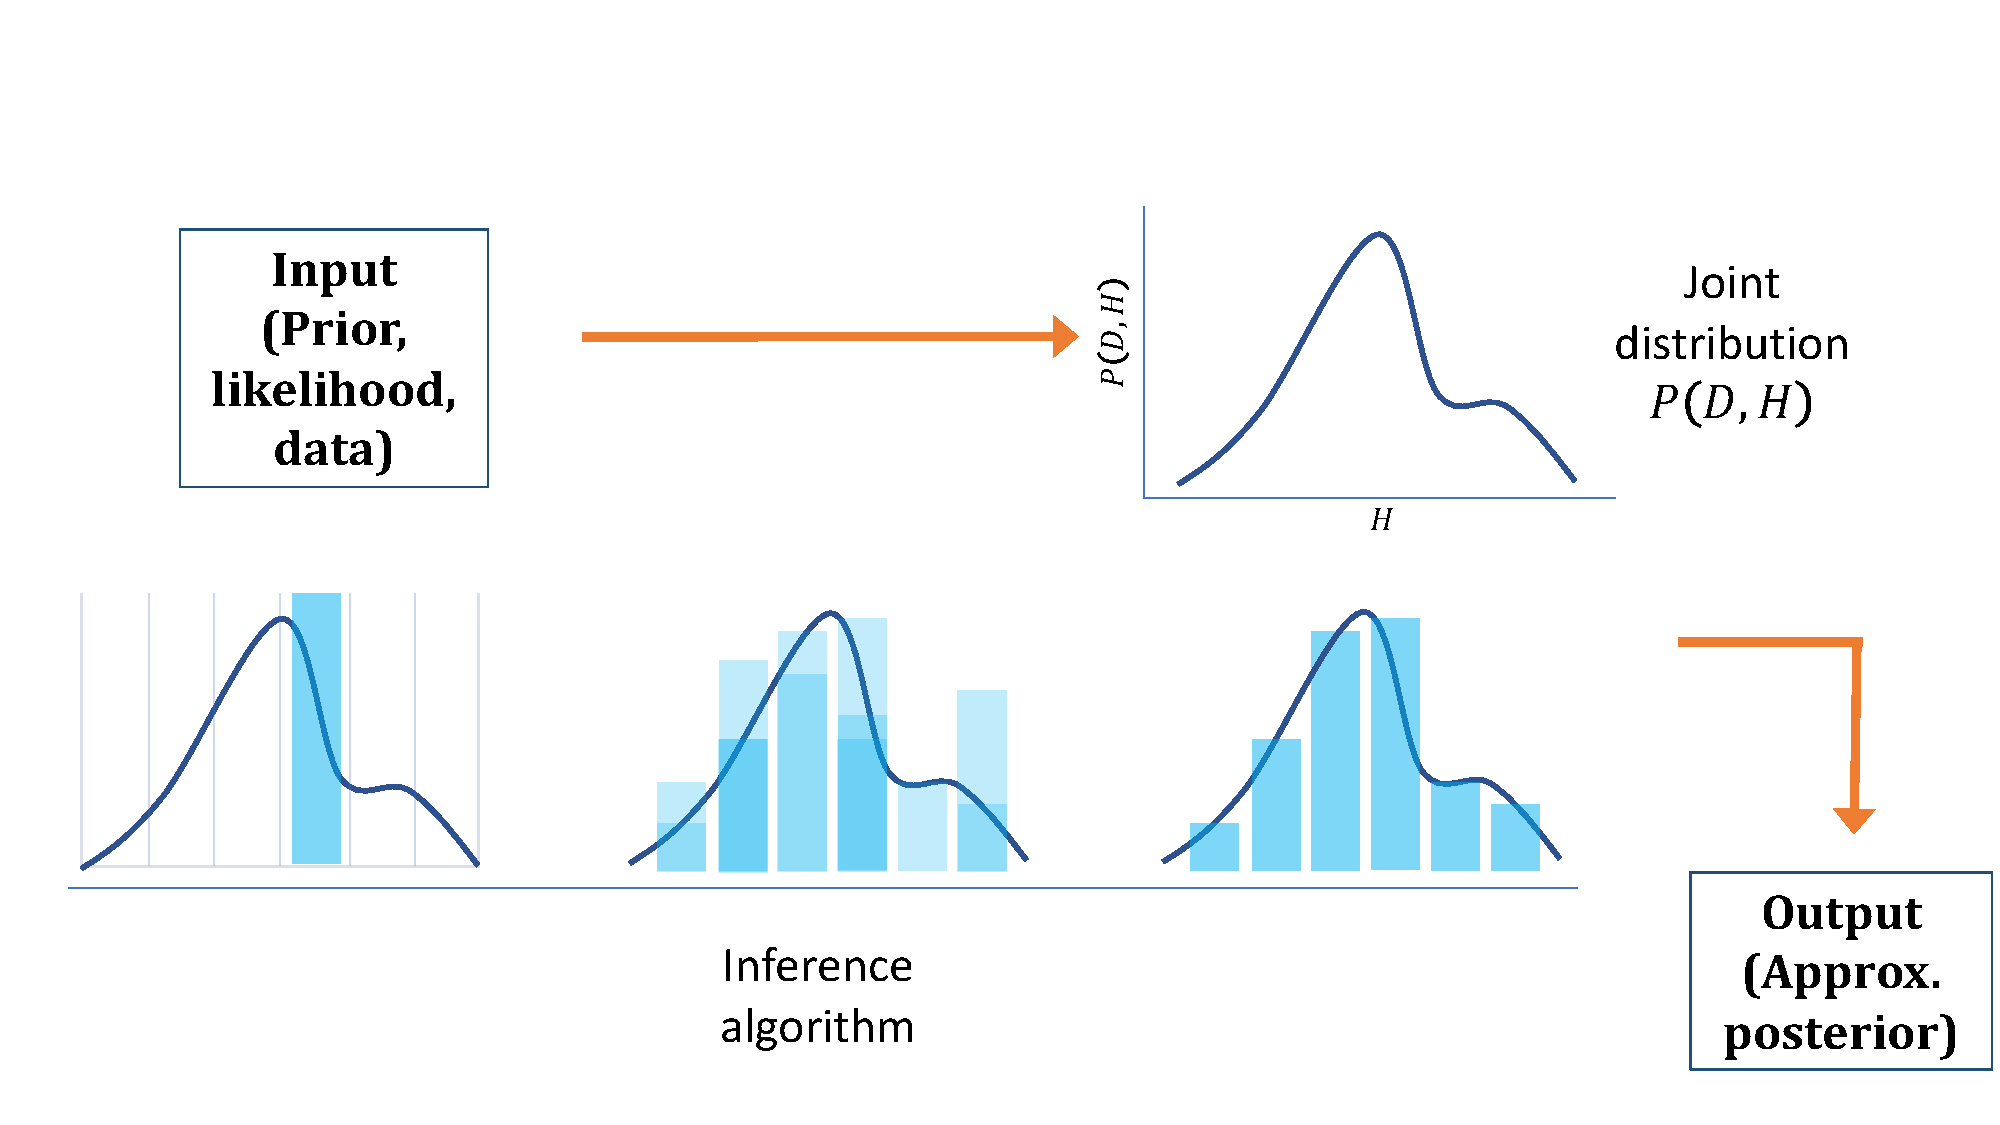
\includegraphics[width = \textwidth]{figures/MonteCarlo_schematic.pdf}
\caption{\textbf{Schematic for Monte Carlo approximation}. }
\label{fig:MC_schematic}
\end{figure}

Sample-based approximations, \citep[also known as \emph{Monte Carlo} approximations][]{robert13}, take the following form:
\begin{align}
P(h|d) \approx \hat{P}_N(h|d) = \frac{1}{N}\sum_{n=1}^N \mathbb{I}[h_n=h]
\end{align}
where $\mathbb{I}[\cdot]=1$ when its argument is true ($0$ otherwise) and $h_n$ is a random hypothesis drawn from some distribution $Q_n(h)$. A schematic is in Figure \ref{fig:MC_schematic}. When $Q_n(h) = P(h|d)$, this approximation is unbiased, meaning $\mathbb{E}[\hat{P}_N(h|d)] = P(h|d)$, and asymptotically exact, meaning $\lim_{N\rightarrow \infty} \hat{P}_N(h|d) = P(h|d)$. This approach is also straightforwardly generalized to sets of hypotheses: $\hat{P}_N(h \in H|d) = \frac{1}{N}\sum_{n=1}^N \mathbb{I}[h_n \in H]$, where $H \subset \mathcal{H}$. 

In general, we cannot directly sample from the posterior, because the normalizing constant $P(d) = \sum_{h} P(h,d)$ requires the evaluation of the joint probabilities of each and every hypothesis and is therefore intractable when the hypothesis space is large. In fact, sampling from the exact posterior entails solving exactly the problem which we wish to approximate. Nonetheless, it is still possible to construct an asymptotically exact approximation by sampling from a Markov chain whose stationary distribution is the posterior; this method is known as \emph{Markov chain Monte Carlo} (henceforth referred to as MCMC). \footnote{There exist other Monte Carlo methods that do not simulate a Markov chain. These include accept-reject methods and importance sampling. While these have the advantage of producing uncorrelated (i.i.d, independent and identically distributed) samples, they do not scale well to high dimensions, and often require pre-existing knowledge of the posterior. This makes MCMC methods the predominant Monte-Carlo method used for Bayesian inference. \cite{neal1993probabilistic, andrieu2003introduction}}

\subsection{Algorithmic details}

In this section I describe a specific variant of MCMC called Metropolis-Hastings. I will briefly also discuss another variant, Gibbs sampling, as a specific case of Metropolis-Hastings.

We assume that the joint distribution is known. Therefore, although we cannot evaluate $P(h | d)$ at any given $h$ since we do not know the normalization factor, we can evaluate relative probabilities between the probabilities of two hypotheses. We also assume a proposal distribution $Q(h)$. We will discuss the importance of the choice of this proposal distribution later in the section. 

The goal is to generate samples from some probability distribution $P(h | d)$. The output therefore should be a set of different hypotheses (denoted $S$) that occur with frequencies determined by $P(h | d)$. This set $S$ determines our sample based approximation $\hat{P}_N(h|d) $. Its size is determined by how many steps $N$ we run the chain for. The procedure we follow is:
\begin{itemize}
\item Start the Markov chain at any random hypothesis $h$. Add it to $S$.
\item Propose a new hypothesis $h'$ by sampling $Q$.
\item Calculate the Metropolis-Hastings acceptance probability $a = \text{min}\left( \frac{P(h' | d) Q(h))}{P(h | d) Q(h')}, 1 \right)$
\item Flip a coin that lands Heads with probability $a$.
\item If the coin lands Heads then accept the proposal $h'$ and add it to $S$. Else reject the proposal and stay at $h$ and add it to $S$ again.
\item Repeat steps 2 onward $N$ times.
\end{itemize}

This results in a Markov chain with $P(h|d)$ as its stationary distribution, see \citet{blitzstein2014introduction} for proofs. As  $N \rightarrow \infty$, the approximation $\hat{P}_N(h|d) $ asymptotically approaches the true posterior $P(h | d)$. See Holden 1998 \cite{holden1998geometric} for proofs.

What remains to be decided is what a good proposal distribution might be. As along as the proposal distribution ensures a finite probability of proposing every state at some point along the chain (ensures \textit{ergodicity}), the samples will converge asympotically to the true posterior. However, the closer the proposal to the true posterior, the faster the algorithm converges on average.\cite{holden1998geometric} The proposal distribution can also depend on the current state of the Markov chain, allowing for local adjustments to the current hypothesis. This often leads to good acceptance probabilities since the posteriors are often smooth -- meaning if a hypothesis has high probability, so will hypotheses that are `close' to it. Another well known variant of MCMC called Gibbs sampling can be seen as a variant of Metropolis-Hastings, with a specific proposal distribution such that the proposals are always accepted. Here the sampling is over a joint distribution over hypotheses $\vec{h}$ that have multiple ($k$) dimensions. The hypothesis along only one of these dimensions $h_i$ is changed in every step, and the proposal distribution is the exact conditional distribution $Q = P(h_i | h_{1:K\setminus i})$. Substituting this into the formula for the acceptance probability, we can see that this proposal is always accepted. The conditional distributions however are not always easy to compute, making Metropolis-Hastings a more general purpose MCMC algorithms (though with the added worry of choosing a good proposal distribution).

\subsection{History}
Sampling methods based on Markov chains were first developed in physics to study properties of the Boltzmann distribution in statistical mechanics. \cite{metropolis1953equation} For a system at equilibrium, the relative frequency of a configuration $\omega$ is given by its Boltzmann weight

\begin{align}
e ^{-E(\omega) / kT}
\end{align}

where $T$ is the temperature and $k$ is the Boltzmann's constant, and $E(\omega)$ is the energy of the configuration $\omega$. The probability distribution over configurations therefore is given by 

\begin{align}
P(\omega) = \frac{ e ^{-E(\omega) / kT}} {Z} = \frac{ e ^{-E(\omega) / kT}} {\sum_{\omega'} e ^{-E(\omega') / kT}}
\label{eq:Boltzmann}
\end{align}

where the denominator $Z$ is called the partition function. This partition function in realistic cases is computationally intractable. This has striking resemblances to the problem of Bayesian inference we described above -- where relative probabilities are easy to compute, but exact probabilities are prohibitive due to the evaluation of an intractable normlizing constant. Some modern MCMC methods like Hamiltonian Monte Carlo\citep{neal1993probabilistic} explicitly form a Hamiltonian, assigning energies to different states, and formulate the probability distribution as a Boltzmann distribution over these states.

The original paper \citet{metropolis1953equation} introduced the \textit{Metropolis} algorithm, where the proposal is limited to being symmetric and local. It was further generalized, and formalized mathematically in \citet{hastings1970monte} to give the modern \textit{Metropolis-Hasting algorithm} described in the previous section.

Versions of MCMC were then applied to optimization problems in the form of \textit{simulated annealing} \cite{kirkpatrick1983optimization}, widening their reach outside of statistical physics. The first Bayesian perspective (as well as a new MCMC algorithm, Gibbs sampling) came from an application of MCMC to the problem of digital restoration\cite{geman1984stochastic}. These methods have since been widely applied in physics, engineering, and artificial intelligence, see \citet{richey2010evolution} for further details on the history of MCMC.


\subsection{Monte Carlo methods in models of cognition}

Sampling theories have long been invoked, implicitly or explicitly, in models of human cognition to justify variation in responses across individuals and trials. In studies demonstrating optimal Bayesian behavior in the average, it has often been found that individual reponses arise from the full range of the distribution, with frequency proportional to the posterior probability, in a phenomena called `probability matching' \citep{wozny2010,Denison2013,Moreno11,Vul2014}. More recently,`rational process models' have explicitly modelled sampling as a mechanism to drive a stronger connection between rational models of cognition and psychological mechanisms \cite{griffiths2012bridging, Vul2014, shi10, sanborn2010rational, Lieder2013, nobandegani2019resource}, see \citet{sanborn2016bayesian} for a review. These highlight phenomena that emerge in the finite sample regime, within a `resource-rational', or computational rationality framework \citep{Vul2014,griffiths2015,Gershman2015,schulz2016simple}: this framework posits that if generating samples is costly (in terms of time and cognitive resources), then the rational strategy is to generate the minimum number of samples necessary to achieve a desired level of accuracy. Such a formalism explicitly bridges the requirements from a computational level account of inference, with the cognitive processes that implement it. \footnote{As discussed in Chapter \ref{chap:psych}, a problem that still impacts these sampling algorithms is of how to know how much to sample. I present a possible solution to optimal stopping (without unrealistic demands on cognitive resources) in Section \ref{sec:MCMC_optimal_stop}.}
%An important implication of this framing is that that incentives or uncertainty should have systematic effects on sample generation. For example, \citet{hamrick2015think} showed that people generated more samples when they were more uncertain. By the same token, cognitive load \citep{sprenger2011} or response time pressure \citep{Dougherty2003} act as disincentives, potentially reducing the number of generated samples.

We have so far discussed the advent of Monte Carlo approximations in cognitive science more broadly, without considering specific algorithms for it. The two main contenders have been importance sampling \cite{shi10} and MCMC \cite{Lieder2013}. In this thesis we discuss MCMC in particular for a few reasons. First, MCMC does not require knowledge of normalized probabilities at any stage and relies solely on an ability to compare the relative probabilities of two hypotheses. It has been shown in the literature \citep{stewart06} that humans have a better sense for relative rather than absolute probabilities. Second, MCMC allows for feedback between the generation and evaluation processes. The evaluated probability of already generated samples influences if and how many new samples will be generated, consistent with adaptive generation of samples like in \citet{hamrick2015think}. Third, Markov chains generate autocorrelated samples, consistent with autocorrelation in hypothesis generation \citep{multistability,vul08,Bonawitz2014}. Correlation between consecutive samples manifested as anchoring effects (where judgments are biased by the initial hypothesis \citep{tversky}) are replicated by MCMC approximations that are also transiently biased (during the`burn-in' period) by their initial hypothesis, prior to reaching the stationary distribution \citep{Lieder2013}. Finally, work in theoretical neuroscience has shown how MCMC algorithms could be realized in generic cortical circuits \citep{buesing11,pecevski11,Moreno11,bernstein2017markov}. In Chapter \ref{chap:MCMC} we discuss in greater detail the unique predictions of MCMC as compared to other sampling algorithms that have been explored in the psychological literature, like importance sampling.
%
%%% Include here?  It doesn't require knowledge of normalized probabilities at any stage and relies solely on an ability to compare the relative probabilities of two hypotheses. This is reassuring because it is much more natural to expect that humans can gauge the relative probabilities of hypotheses better than their absolute probabilities \citep{stewart06}.
%%ERIC: Just as a side note, I'm not sure if the Stewart paper is the normal reference for that. Absolute vs relative probabilities goes all the way back to Kahneman vs. Gigerenzer
%
%To highlight the distinctive predictions of MCMC, it is useful to compare it with other sampling algorithms that have been explored in the psychological literature. \emph{Importance sampling} also uses a proposal distribution $Q(h)$, but unlike MCMC it samples multiple hypotheses independently and in parallel. These samples are then weighted to obtain an approximation of the posterior:
%\begin{align}
%\hat{P}_N(h|d) = \frac{1}{N} \sum_{n=1}^N \mathbb{I}[h_n=d] w_n,
%\end{align}
%where $w_n$ is an ``importance weight'' for sample $n$ computed according to:
%\begin{align}
%w_n \propto \frac{P(h_n,d)}{Q(h_n)}.
%\end{align}
%Intuitively, the importance weight corrects for the fact that the importance sampler draws samples from the wrong distribution. \citet{shi10} have shown how this algorithm can be used to simulate human performance on a wide range of tasks. They also identified a correspondence between importance sampling and exemplar models, which have been widely applied in psychology. In related work, \citet{shi2009neural} demonstrated how importance sampling could be realized in a biologically plausible neural circuit \citep[see also][]{abbott13}.
%
%Some of the effects we have replicated in this work could also be captured by an importance sampling algorithm with limited samples. \citet{Thomas2008} have proposed a model, HyGene, that is similar in spirit to an importance sampler with limited samples, with a memory driven proposal distribution that selects the hypotheses to be generated. HyGene explains subadditivity in terms of a failure to retrieve all the relevant hypotheses from memory due to stochastic noise in the retrieval process and limited working memory capacity.
%
%The self-generation effect can to some extent be reproduced by importance sampling because prompting a hypothesis causes it to be sampled an extra time. So the probability of the focal space will be slightly larger if hypotheses in it are explicitly prompted (other-generated and presented to the participant) than if it they are generated without prompting (self-generated). However, Experiment 2 in \cite{conf} shows that in a situation where all the alternatives are specified, prompting specific hypotheses (as in the other-generated scenarios), does not result in a higher probability judgment than when these hypotheses are not prompted (as in the self-generated scenarios). The MCMC algorithm captures this finding because in a small hypothesis space, the Markov chain will visit all the hypotheses with the right frequency irrespective of initialization. By contrast, the importance sampler predicts a higher probability for other-generated hypotheses, contrary to the empirical finding.
%
%This brings us to a key difference between importance sampling and MCMC: Importance sampling generates all hypotheses in parallel---the generation of new hypotheses has no dependence on hypotheses that have already been generated. Without this dependence, there is no interaction between the generation and evaluation processes. MCMC captures this dependence by sequentially generating hypotheses. Our model's explanation of the self-generation effect, superadditivity, the weak evidence effect and the dud alternative effect rests on this dependence. The Markov chain can get `stuck' (at least temporarily) by rejecting proposals, thus generating fewer alternatives. If, on the other hand, the current hypothesis has low probability, more alternatives are generated and the probability estimate of the focal space is reduced.
%
%The important sampler does not produce these effects, because its mechanism for generating new hypotheses is independent of the probability of the current one. If anything, prompting a hypothesis within the focal space, no matter how atypical, causes it to be sampled, \textit{increasing} the importance sampler's estimate for the probability of the focal space, contradicting superadditivity.
%
%Another key difference between MCMC and importance sampling is that MCMC generates correlated samples, whereas consecutive samples from an importance sampler are totally independent. This prevents the importance sampler from reproducing the effects in Table \ref{tab:biases} that rely on correlated sampling, such as the anchoring effect and the crowd within.
%
%Importance sampling has also been adapted to inference in dynamical systems by generating hypotheses online---a technique known as \emph{particle filtering}. This approach has been fruitfully applied to a number of domains in psychology, such as multiple object tracking \citep{vul2009explaining} and change detection \citep{brown09}. Although hypotheses are generated sequentially by particle filtering, it is important to note that this structure is dictated by the sequential nature of the generative process. For example, in multiple object tracking, the object positions are dynamic latent variables; particle filtering generates new hypotheses about the positions after each new data point is observed. In contrast, the sequences of hypotheses generated by MCMC algorithms are purely mental, in the sense that hypotheses are generated sequentially regardless of whether the generative process is itself sequential. In this paper, we focus on non-sequential generative models in order to stress this point.
%
%

\section{Variational methods}
\label{sec:approx_var}


\begin{figure}
\centering
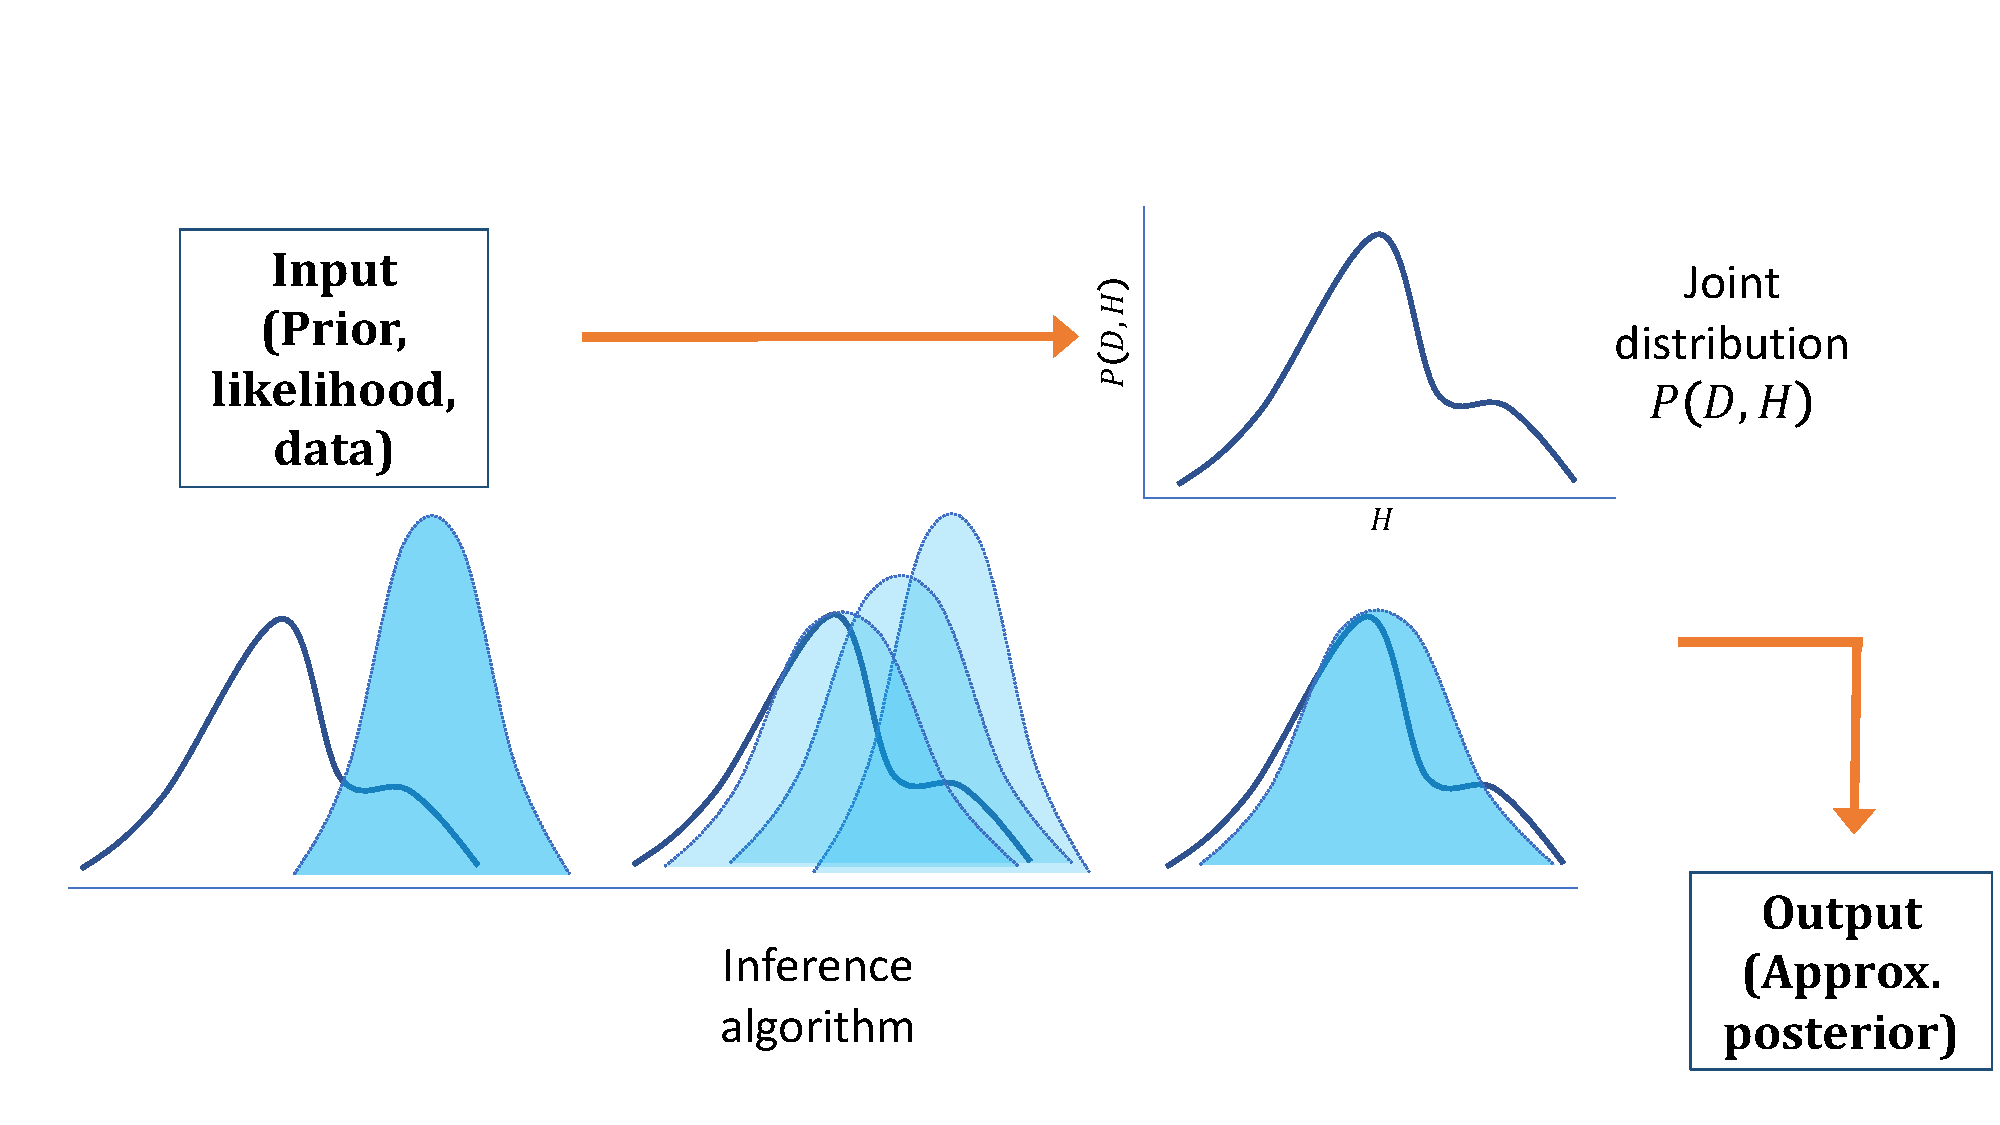
\includegraphics[width = \textwidth]{figures/variational_schematic.pdf}
\caption{\textbf{Schematic for Variational approximation}. }
\label{fig:var_schematic}
\end{figure}


To motivate variational approximations, we first consider a more general case of Monte Carlo approximation, using weighted samples
\begin{align}
    P(h|d) \approx \sum_{n=1}^N w^n \mathbb{I}[h^n = h],
    \label{eq:montecarlo}
\end{align}
Monte Carlo algorithms can be thought of as procedures for generating an approximate posterior $Q_\phi(h|d)$ parametrized by the set of these weights and samples, $\phi = \{ w^n, h^n \}_{n=1}^N$. In MCMC, these weights are always one, but methods like importance sampling posit non-unit weights. The superset $\Phi$ of all feasible sets (i.e., the sets that can be produced by a particular Monte Carlo algorithm) is defined as the approximation family of this algorithm. This allows us to formalize a more general view of approximate inference as an optimization problem: find the approximation (parametrized by $\phi \in \Phi$) that gets `closest' to the true posterior, where dissimilarity between the two distributions is measured by a divergence functional $\mathcal{D}$. 
\begin{align}
\phi^\ast = \argmin_{\phi \in \Phi} \mathcal{D}[Q_\phi(h|d)||P(h|d)],
\end{align}
Monte Carlo algorithms do not solve this optimization problem, but instead randomly sample $\phi$ such that, in the limit $N \rightarrow \infty$, they produce $\phi^\ast$. It is however possible to design non-randomized algorithms that directly optimize $\phi$ even in a sample-based approximation\citep{saeedi2017variational} and in fact form the basis for optimal stopping in sampling-based rational process models discussed in Section \ref{sec:MCMC_optimal_stop}. Such optimization is an example of \emph{Variational Inference} \citep{jordan1999introduction}.

The general idea of Variational Inference (VI) is to first posit a family of densities and then to find a member of that family which is closest to the target probability distribution. Classic variational methods use the \textit{Kullback-Leibler} divergence (also known as relative entropy) as a measure of closeness. This is given by:
\begin{align}
\mathcal{D}_{\text{KL}}[Q_\phi(h|d)||P(h|d)] = \sum_h Q_\phi(h|d) \log \frac{Q_\phi(h|d)}{P(h|d)}.
\end{align}
This formulation reduces the problem of approximate inference to an optimization problem to which any standard algorithm for optimization may be applied. An example with a Gaussian approximation family and an iterative optimization procedure is given in Figure \ref{fig:var_schematic}.

In general however, this divergence cannot directly be optimized, since finding a $Q$ that optimizes $\mathcal{D}_{\text{KL}}$ requires knowing the exact $P$. We of course cannot already know the exact $P$, since it is precisely the distribution we are trying to approximate. Instead we optimize an alternative objective that is equivalent to $\mathcal{D}_{\text{KL}}$ up to an added constant. This is called the \emph{evidence lower bound} (ELBO) and is given as follows:

\begin{align}
\text{ELBO}[Q_\phi(h|d)] &=  \sum_h Q_\phi(h|d) \log \frac{P(h,d)}{Q_\phi(h|d)}  \nonumber \\
& = \sum_h Q_\phi(h|d) \log \frac{P(h|d)}{Q_\phi(h|d)} + \sum_h Q_\phi(h|d) \log P(d)  \nonumber \\
& = - \mathcal{D}_{\text{KL}}[Q_\phi(h|d)||P(h|d)]  + \log P(d)
\label{eq:ELBO}
\end{align}

This function is  also known as the negative variational free energy. The term ELBO comes from the fact that $\mathcal{L}[Q_\phi(h|d)]$ is a lower bound on the `evidence' (log marginal likelihood) $\log P(d)$, since a KL divergence between any two distributions is restricted to be greater than or equal to zero. Since the evidence in a specific situation is fixed, maximizing the ELBO will produce the same variational approximation as minimizing the KL divergence. Critically, the ELBO eliminates the dependence on $P(h|d)$, only requiring access to the unnormalized posterior, the joint distribution $P(h,d)$.


\subsection{Algorithmic details}
\label{sec:var_alg}

Algorithms for variational inference vary on two dimensions. First, the specific variational family we use can vary, and how good of a fit it is to the aspects of true posterior that we wish to capture. Unlike MCMC, variational inference does not have any formal guarantees about asympotically reaching the true posterior -- for example, if the variational family chosen does not actually contain the true posterior, the variational approximation never converge to the exact distribution. Different choices of the approximation family can give vastly different approximations. Second, the optimization algorithm used can vary. This also interacts with the choice of variational family -- with the goal of allowing maximum complexity in the variational family while managing the complexity of performing the optimization effectively. Note that exactly computing the ELBO (Equation \ref{eq:ELBO}) still requires an expectation over $Q_\phi$ which may not always be tractable, and may need to be approximated. This makes optimizing even the ELBO a non-trivial problem.

In this section we concentrate on one approach to variational inference. We use deep neural networks as flexible function approximators \citep{dayan1995helmholtz,kingma2014auto,mnih2014neural,rezende2015variational,paige2016inference}, and optimize the parameters of these networks (as the variational parameters). This allows us to leverage the developments made in gradient based optimzation of such architectures. The idea is that the network takes in the relevant information about the data $d$ that we want to condition on and produces some output. These outputs can be interpreted as the traditional notion of `parameters' of a variational family $\phi$ -- for example if we were considering a Gaussian variational family then the outputs could be the mean and variance. However, these `parameters' are produced by the parameters of the neural network, and we can directly optimize these network parameters instead, utilizing much of the progress made in recent years in efficiently and scalably training neural networks. Another advantage of this approach is the ease of \textit{amortization}, which is discussed in further detail in Chapter \ref{chap:LTI}.

Even given the ease of gradient-based optimization of neural network architectures (using the backpropagation algorithm), we still need to first find the gradient of the cost function (the ELBO) with respect to our variational parameters. We describe an approximate technique for optimizing the ELBO known as \emph{blackbox variational inference} \citep{ranganath2014black} where we directly approximate the gradient of the ELBO with respect to our variational parameters. This still requires the computation of an expectation over $Q_\phi$, which is tractably approximated with a set of $M$ samples:
\begin{align}
    \nabla_\phi \text{ELBO}[Q_\phi(h|d)] \approx \frac{1}{M} \sum_{m=1}^M \nabla_\phi \log Q_\phi(h^m|d) \left[ \log P(h^m,d) - \log Q_\phi(h^m) \right],
\end{align}
where $h^m \sim Q_\phi(h|d)$. Using this approximation, the variational parameters can be optimized with stochastic gradient descent updates of the form:
\begin{align}
    \phi_{t+1} \leftarrow \phi_t + \rho_t \nabla_\phi \text{ELBO}[Q_\phi(h|d)],
\end{align}
where $t$ indexes iterations and $\rho_t$ is an iteration-dependent step-size. Provided $\rho_t$ satisfies the Robbins-Monro stochastic approximation conditions ($\sum_{t=1}^\infty \rho_t = \infty, \sum_{t=1}^\infty \rho_t^2 < \infty$), this optimization procedure will converge to the optimal parameters with probability 1.

\subsection{History}

The history of variational inference is more difficult to trace since it is a broader concept intimately tied to the history of optimization. Some of the first variational approximations, recognizable as such, appear in statistical physics as mean field theories. The first of these was the Curie-Weiss theory for ferromagnetism, that made a mean-field approximation to the Ising model\cite{curie1895proprietes,  weiss1907hypothese}. Here, the local field at each point on a lattice is approximated by a global field that applies uniformly to the whole lattice. This effectively ignores correlations between the lattice sites. In the language of probability distributions this constitutes approximating the probability distribution $P(\vec{h} | d)$ defined over a potentially complex joint distribution over the $K$ dimensions of $\vec{h}$ (the magnetizations at different lattice sites for example), with a factorized distribution $Q_\phi$ where
\begin{align}
Q(\vec{h}| d) = \prod_{i}^K Q_{\phi_i}(h_i | d)
\end{align}
The parameters $\phi_{1:K}$ defining the parameters of the variational family are then optimized. Here, the correlations between the different dimensions are neglected. Subsequent to this model, several other mean field theories were developed across other domains of physics. Following these, \citet{landau1965collected} formalized mean field theory as a variational approximation\cite{kadanoff2009more}. Concurrently, variational approaches were also applied to problems in quantum physics and quantum field theory \citep{milton2006electromagnetic, feynman1965quantum}.

Variational approaches are also used in statistical physics in the context of the partition function problem discussed in the section on sampling\citep{kikuchi1951theory, bethe1935statistical}. While Markov chain Monte Carlo can simulate samples from unnormalized Boltzmann distributions (Equation \ref{eq:Boltzmann}), and thereby provide normalized probabilities, sampling methods cannot provide an actual value for the normalization constant or partition function $Z$. The negative logarithm of this partition function is the free energy. By the principle of minimizing energy, equilibrium states in physical systems will minimize this free energy. The logarithm of this partition function is also the log marginal likelihood of the data, or the `evidence' in the language of probabilistic inference. We can use variational inference to to approximately minimize this free energy, by instead maximizing the ELBO (the lower bound to the evidence). 

The development of variational methods specifically for Bayesian inference arguably started with a mean field learning algorithm for neural networks in \citet{anderson1987mean}, followed by formalization of variational approximations to a slew of other models\citep{saul1996mean, jaakkola1997variational}. These approaches have been extensively studied in statistics and machine learning, and provide a strong alternative to MCMC for scalable posterior approximation \citep{blei2017variational, jordan1999introduction}.

Variational methods have been evoked in models of human cognition both implicitly and explicitly. Certain models of human perception\cite{lau2018ensemble} and associative learning\cite{gershman2015unifying} make implicit assumptions about what moments of a distribution humans track -- in some cases these can be interpreted as a variational approximation with a Gaussian family. Studies of cognition that invoke the Free Energy Principle via the notion of active inference\cite{friston2015active}
%-- the idea actions are directed not only to maximise external reward, but also maximise information gain -- 
explicitly claim a variational framework. This approach to approximate inference has also been studied from a neuroscience perspective, where its appeal lies in allowing us to contemplate complex, biologically realistic approximation architectures (provided that the optimization procedures can also be realized biologically; see \citet{whittington2019theories}). For example, particular implementations of variational inference have been used to model hierarchical predictive coding in the brain \citep{friston2008hierarchical,gershman2019does}.


\section{Hybrid methods}
%
%%Our theory relies heavily on a variational framework for thinking about the optimization problem that is being solved by the brain's approximate inference engine. This creates some dissonance with prevailing ideas about approximate inference in cognitive science, most of which have been grounded in a hypothesis sampling (Monte Carlo) framework \citep[see][for a review]{sanborn2016bayesian}, with small numbers of samples. Hypothesis sampling has also been studied independently in neuroscience as a biologically plausible mechanism for approximate inference \citep[e.g.,][]{buesing2011neural,haefner2016perceptual}. In our own prior theoretical work, we have employed hypothesis sampling to explain a range of inferential errors \citep{dasgupta2017hypotheses,dasgupta2018remembrance}. 

Sampling methods like MCMC and variational methods usually trade-off in expense vs precision. MCMC can be very slow to converge, in particular when the parameters being inferred are high dimensional. Each sampling step can be expensive if we are conditioning on a very large data-set. However, they come with an asymptotic guarantee -- if the algorithm is run for long enough, the approximation converges to the true posterior. On the other hand, variational methods are much cheaper. Optimization is fairly well understood problem with many advances in improving convergence speed. With stochastic approaches to this optimization problem, each step of the optimization can also be made very easy. We also reserve a lot of flexibility in how good of an approximation we want by choosing how expressive our variational family is.  However, the convergence of this optimization does not guarantee that we have reached the true posterior. Several recent methods in the machine literature combine the complementary advantages of these approximation method leading to several new algorithms \citep{li2017approximate, naesseth2017variational, ruiz2019contrast}. These two approaches also have different characteristics when considering amortization or re-use of inference, we discuss this briefly in Chapter \ref{chap:amort}. 

Prevailing ideas about approximate inference in cognitive science are largely grounded in a hypothesis sampling Monte Carlo framework (see \citet{sanborn2016bayesian} for a review), with small numbers of samples. In this thesis, I introduce a variational approach in Chapter \ref{chap:LTI} and how it can expand the scope of rational process models by providing a framework for the flexible re-use of computation. Below, I discuss a few concrete possibilities for how sampling and variational approaches might be combined to build new, testable models of human probabilistic inference.

\subsection{Proposal distribution}

Almost all Monte Carlo methods rely on a proxy distribution for generating samples. Markov chain Monte Carlo methods construct a Markov chain whose stationary distribution is the true posterior, often making use of a proposal distribution to generate samples that are accepted or rejected. Importance sampling methods simultaneously draw a set of samples from a proposal distribution and reweight them. Particle filtering methods apply the same idea to the case where data are observed sequentially. One natural way to combine variational inference with these methods is to use the variational approximation as a proposal distribution. This idea has been developed in the machine learning literature e.g. in \citet{de2001variational,gu2015neural}, but has not been applied to human judgment.

For Markov chain Monte Carlo methods, another possibility would be for the variational approximation to supply the initialization of the chain. If enough samples are generated, the initialization should not matter, but a number of cognitive phenomena are consistent with the idea that only a small number of samples are generated\citep{vul2014one}, thereby producing sensitivity to the initialization. For example, probability judgments are influenced by different ways of unpacking the sub-hypotheses of a disjunctive query \citep{dasgupta2017hypotheses} or providing incidental information that serves as an `anchor' \citep{lieder2017anchoring,lieder2018empirical}. In these studies, the anchor is usually provided as an explicit prompt in the experiment -- variational approximations could provide such an anchor for a new query in the absence of an explicit prompt.

The quality of the proposal distribution as well as the sampled initialization (in terms of its proximity to the true posterior) determines the speed of convergence of a sampling algorithm\citep{holden1998geometric}. We will see in Chapter \ref{chap:MCMC} how an un-converged sampling approximation can explain several cognitive biases. Variational inference provides a mechanism for learning a good proposal distribution or initialization over time. Using this within a sampling framework could explain why people show different degrees of biases in different domains, despite similarity in cognitive resources, i.e. a similar number of samples.

\subsection{Optimal stopping}
\label{sec:MCMC_optimal_stop}

The computational rationality perspective on sampling argues that the number of samples is chosen adaptively to balance the benefits of taking more samples against their costs in time and energy \citep{Gershman2015,Vul2014,griffiths2015}. To find the optimal stopping point, we need to compute the value of additional samples, and decide whether it outweighs the cost of taking these additional samples. A naive approach to finding the value of additional samples is to examine how much closer this gets us to the true posterior distribution. This however is circular, since the true posterior is what we are trying to approximate in the first place. So we cannot compare our current approximation against it. I discussed this problem in Chapter \ref{chap:psych} in Section \ref{sec:psych_BR}, when considering concerns with current models of resource-rationality or computational rationality -- that knowing the optimal stopping point, in the most naive sense, can be more expensive that the original computation we set out to approximate. 

There are however ways to get around this for certain classes of rational-process models, including the sampling mechanism proposed in this thesis in Chapters \ref{chap:MCMC} and \ref{chap:MCMC_amort}. To understand this, we first formalize the boundedly rational cost function. If the approximate posterior is given by

\begin{align}
P(h|d) \approx \hat{P}_N(h|d) = \frac{1}{N}\sum_{n=1}^N \mathbb{I}[h_n=h],
\end{align}

Then the bounded rationality objective function is a function of the distance $\mathcal{D}$ between this approximation and the true posterior, as well as the cost of the resources required to make this approximation. We assume that cost scales linearly with the number of samples, with $\mathcal{C}$ per sample. This gives the following objective $\mathcal{F}$ that we wish to minimize as a function of the number of samples (N):
\begin{align}
\mathcal{F}(N) = \mathcal{D}[\hat{P}_N(h|d)||P(h|d)] + \mathcal{C}N
\end{align}
We choose the Kullback-Liebler (KL) divergence, or relative entropy, as the distance metric to get
\begin{align}
\mathcal{F}(N) &= \mathcal{D_{KL}}[\hat{P}_N(h|d)||P(h|d)] + \mathcal{C}N \\
& =  \sum_h \hat{P}_N(h|d) \log \frac{\hat{P}_N(h|d)}{P(h|d)} + \mathcal{C}N
\end{align}
Exactly computing this objective still requires the exact posterior to evaluate exactly. However, two insights make this tractable. First, we note that the KL divergence can we written as follows (see also Equation \ref{eq:ELBO}):
\begin{align}
\mathcal{D_{KL}}[\hat{P}_N(h|d)||P(h|d)]  = \sum_h \hat{P}_N(h|d) \log \frac{\hat{P}_N(h|d)}{P(h,d)} + \log P(d)
\label{eq:split_KL}
\end{align}
Here, the first term is computable since a) we know the joint distribution $P(h,d)$,  and b) we can take expectations over our approximate distribution $\hat{P}_N(h|d)$. The second term (the evidence or negative free energy) remains intractable. 

However, our second insight is that we do not need to compute the exact value of the objective function. Our objective function is a linear sum of smooth monotonic functions: the KL term decreases (on average) with increase in the number of samples, and the cost term increases. Therefore, our cost function is convex, and the global minimum can be found simply by following local gradients. This smooth, convex assumption does not hold for many other classes of resource-rational approximations, for example, if we are optimizing over the space of discrete strategies (eg. whether to employ a certain heuristic or another), rather than optimizing over an (almost) continuous parameter like the number of samples drawn. This local gradient (or the incremental value to one additional sample) is given by:
\begin{align}
\mathcal{F}(N + 1) - \mathcal{F}(N) =  \sum_h \hat{P}_{N+1}(h|d) \log \frac{\hat{P}_{N+1}(h|d)}{P(h|d)} -  \sum_h \hat{P}_N(h|d) \log \frac{\hat{P}_N(h|d)}{P(h|d)} + \mathcal{C}
\end{align}
Since the second term in Equation \ref{eq:split_KL} is the same in both, it cancels out, leaving a tractable expression for the gradient. The gradient can therefore be estimated locally everytime a new sample is drawn. Once this gradient starts to become negative, it is time to stop computations. This can be seen as treating the sample based approximation as a variational family and finding the optimal number of samples\cite{saeedi17}, pointing to another important way in which sampling methods and variational methods can be combined to give more complete models of human probabilistic inference.

%See Chapter \ref{chap:approx}, Section \ref{sec:approx_var} for further details on variational approximations.

%
%% consisting of a handful of samples in response to the current query. We discussed in broader terms the potential role of a learned inference model in augmenting predictions from a noisy sampler as part of our section on `Amortization as Regularization'.

%Almost all Monte Carlo methods rely on a proxy distribution for generating samples. Markov chain Monte Carlo methods construct a Markov chain whose stationary distribution is the true posterior, often making use of a proposal distribution to generate samples that are accepted or rejected. Importance sampling methods simultaneously draw a set of samples from a proposal distribution and reweight them. Particle filtering methods apply the same idea to the case where data are observed sequentially. One natural way to combine variational inference with these methods is to use the variational approximation as a proposal distribution. This idea has been developed in the machine learning literature \citep[e.g.,][]{de2001variational,gu2015neural}, but has not been applied to human judgment.
%
%For Markov chain Monte Carlo methods, another possibility would be for the variational approximation to supply the initialization of the chain. If enough samples are generated, the initialization should not matter, but a number of cognitive phenomena are consistent with the idea that only a small number of samples are generated, thereby producing sensitivity to the initialization. For example, probability judgments are influenced by different ways of unpacking the sub-hypotheses of a disjunctive query \citep{dasgupta2017hypotheses} or providing incidental information that serves as an `anchor' \citep{lieder2017anchoring,lieder2018empirical}. In these studies, the anchor is usually provided as an explicit prompt in the experiment -- variational approximations could provide such an anchor for a new query could be in the absence of an explicit prompt.

%
%The blackbox variational inference algorithm that we use described in the (Section \ref{sec:var_alg}) does in fact involve sampling: the gradient of the evidence lower bound is approximated using a set of samples from the variational approximation. Although we are not aware of direct evidence for such an algorithm in brain or behavior, the idea that hypothesis sampling is involved in the learning process is an intriguing possibility that has begun to be studied more systematically \citep{bramley2017formalizing,bramley2018grounding,rule2018learning}. It resonates with work in other domains like reinforcement learning, where people seem to engage in offline simulation to drive value updating \citep{gershman2014retrospective,gershman2017imaginative,momennejad2018offline}.
%
